\chapter{Reorganization of network architecture during reading}

\section{Motivation}

\begin{itemize}
	\item Resting-state is useful, modularity is sensitive, better readers have more modularity, auditory/CON modularity is anti-correlated with reading skill
	\item Our argument is that higher modularity indexes greater flexibility -- more efficient. This should be reflected during tasks.
	\item How does the brain re-organize during tasks? How is this reflected in our connectome measures? Is there a relationship between "participation" and activation?
	\item Are individual differences sensitive to re-organization? Are better readers combining networks more? (No)
	\item What network relationships are changing during reading, compared to rest? Are better readers showing more or less difference? Are there patterns in this change (within-network vs. between-network relationships?)

	\item Across a variety of tasks, is it advantageous to have high ``flexibility'' of global network states? 
	\begin{itemize}
		\item Similarity between listening and reading network architecture will correspond to higher reading skill.
		\item Dissimilarity between language comprehension tasks and other tasks will correspond to higher reading skill.
	\end{itemize}

\end{itemize}

Resting-state functional connectivity is thought to provide insights into a relatively stable, ``intrinsic'' architecture. This is related to some degree to other aspects of brain structure, including structural connectivity via white matter tracts and cortical thickeness and folding \citep{}. In Study 1, we found that global modularity is positively related to reading skill, even when controlling for verbal intelligence and motion. The inference is that global modularity is indicative of a brain organization that is more ``tuned'' to pass the information between the disparate systems needed for reading. 

% Reorganization during tasks is importpant
However, it is also known that the brain can reconfigure to address new challegnes in the environment, including those of reading. It has previously been seen that, although there are many similarities within the network connectivity during rest, there also differences that arise due to task activity. 

According to one line of reasoning, the ``small-world'' architecture should provide a relatively stable platform for integrating multiple different areas. 
% In this study, we related intrinsic, resting state network organization to reconfigured network organization during the performance of two tasks: a sequence tapping task, which is thought to probe motor execution and likely engages a single brain network, and an n-back task, which is thought to probe working memory and likely requires coordination across multiple networks. We implemented graph theoretical analyses using functional connectivity data from fMRI scans to calculate whole-brain measures of network organization in healthy young adults. We focused on quantifying measures of network segregation (modularity, system segregation, local efficiency, number of provincial hub nodes) and measures of network integration (global efficiency, number of connector hub nodes). Using these measures, we found converging evidence that local, within-network communication is critical for motor execution, whereas integrative, between-network communication is critical for working memory. These results confirm that the human brain has the remarkable ability to reconfigure its large-scale organization dynamically in response to current cognitive demands and that interpreting reconfiguration in terms of network segregation and integration may shed light on the optimal network structures underlying successful cognition. \citep{CohenEsposito}. 



First, we validate modularity and participation coefficient metrics using univariate data, and test that language induces greater global integration, especially in higher-order networks (executive and attention) compared to resting and attention baselines. Second, we test three hypotheses about how interactions between brain networks might differ from speech.


\section{Methods}

\subsection{Participants}

Participants were drawn from the same cohort of subjects included in Study 1, and identical inclusion criteria for both demographic and scan motion were applied. However, additional measures related to the performance of the task were levied as described below. A total of 47 unique subjects and 88 scan sessions were included in the analysis. Their demographics are described in Table \ref{table:ch3-participants}.

\begin{table}
	\renewcommand{\tabcolsep}{0.09cm}
	\centering
	\begin{tabular}{lc}
\toprule 
Measure & Subjects \\ 
\midrule 
No. Participants				& 42 \\ 
No. Scan Runs					& 164 \\ 
Gender  						& 25 F \\ 
Age at Scan 					& 10.5 (0.3)  \\ 
WASI Full-Scale IQ  			& 111.0 (16.2) \\ 
TOWRE - Total Word Efficiency 	& 104.6 (18.5) \\ 
\bottomrule 
\end{tabular}
	\caption[Participant demographics for Study 2.]{Participant demographics for Study 2. Subjects include all of those from Study 1.}
	\label{table:ch3-participants}
\end{table}


\subsection{MRI acquisition and task design}

Functional MRI acquisition parameters were identical to Study 1 with the exception of duration: a total of 250 dynamic volumes were collected for each scan session. During the MRI scan session, participants performed up to four runs of a language comprehension task, which was crossed on two conditions: the modality of presentation (listening or reading) and the passage genre (expository or narrative).  

For the present analysis, only the ``reading'' scans are considered, and the effects of genre on brain activation are ignored, as they are mostly balanced out within subject. In the following paragraphs, however, we will describe the experiment design in its entirety, as it will be relevant to subsequent analyses.

Each fMRI run had two baseline conditions: a modality-specific baseline task and a resting-state block with a fixation cross. At the conclusion of the comprehension portion of each experiment, two images were presented and subjects were asked to decide if the image was related to the passage. (e.g., Is a picture of a cake with candles related to a story about a birthday party?) The order and duration for each block varied slightly across runs but was approximately: paragraph 1 (60 s), baseline 1 (60 s), paragraph 2 (60 s), baseline 2 (60 s), and resting-state (270 s). Total scan time was 550 s for each run. See Fig. \ref{fig:ch3-task-design} for a schematic describing one of the tasks.

\begin{figure}[t]
	\centering
	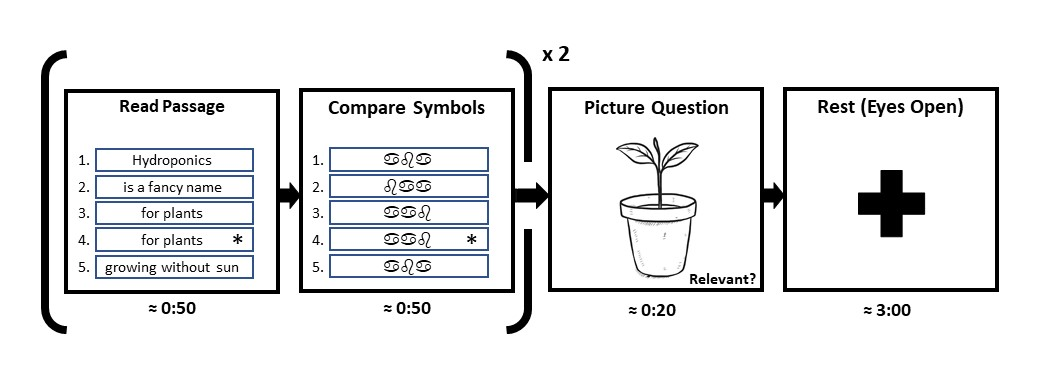
\includegraphics[width=6in]{ch3-task-design}
	\caption[Schematic of the reading comprehension task.]{Schematic of the reading comprehension task. }
	\label{fig:ch3-task-design}
\end{figure}

To create a more naturalistic reading experience than single word presentation \citep{Rayner1998}, passages were presented in syntactic phrases ranging from 1-7 words in length. The interval between each stimulus was jittered to allow for event-related analyses (range: 275 – 4000 ms), although these effects were not examined here.

The sensory baseline condition was altered according to modality. For the reading runs, three non-alphanumeric symbols were displayed horizontally (two types), and their presentation time was matched to the passage phrases. Spacing between symbols was randomly alternated to replicate the variable phrase lengths in the passage condition. For the listening runs, three tones (two frequencies) were played in sequence, with a new set of tones beginning at the same intervals as the corresponding passage presentation. 

To monitor attention, 4 to 8 percent of the stimuli within each passage or attention block were randomly repeated on two consecutive screens.  Participants pressed a button with their right thumb when they detected a repeated phrase, symbol or tone configuration. Additionally, at the conclusion of each passage, a picture was presented on the screen, and subjects were asked to identify whether the picture had any relationship to the passage (e.g., a picture of a mushroom for a passage about fungi). 

To assess performance, we analyzed three measures: in-scanner attention, in-scanner comprehension, and post-scan recall. To assess attention, we calculated the $D`$ statistic ($Z(true\ positive) - Z(false\ positive)$) for the "repeated stimulus" task. The in-scanner comprehension measure was the number (0,1,2) of questions correclty answered. To assess recall, each child was asked to recite as much of the passage as they could remember, and their answers were mapped to actual phrases present in the chapter. Individual scan runs with a $D`$ value less than 2 were excluded from analysis.

In total, there were 4 passages (2 listening, 2 reading), each leveled to a 3\textsuperscript{rd} grade difficulty and balanced on word measures such as concreteness and cohesiveness.  All subjects were trained on the task in a mock scanner prior to the actual scan. 


\subsection{Activation analyses}

Whole-brain fMRI analyses were performed using tools from the FMRIB Software Library (version 5.0.9). For each session, the following pre-processing steps were performed:  slice-time correction, motion correction to the initial fMRI volume, high-pass filtering at 0.08 Hz, boundary-based registration to the subject's structural image, and normalization to 2 mm MNI 152 standard space. To mitigate the effects of motion on our analyses, we regressed out 6 continuous motion parameters and scrubbed out outlier volumes. We defined an outlier volume as any in which the root-mean-square framewise displacement exceeded 0.7 mm. Because head motion can be a major confound for connectivity analyses, we removed scan runs where more than 10 percent of the fMRI volumes were outliers.

All task conditions were convolved with the double-gamma hemodynamic response function to generate design matrices for each fMRI run. Two first-level contrasts were of interest: the main effect of passage comprehension (``Reading vs. Rest''), and the contrast of passage comprehension vs. the sensory baseline (``Reading vs. Attention''). Repeated stimuli and the picture comprehension task were modelled out.

Reading effects were estimated at the subject-level using fixed effects analysis. These were carried over into group-level analyses using non-parametric methods implemented in FSL’s \textit{randomise} tool with threshold-free cluster enhancement. For each group-level analysis, we performed 5000 permutations and report results with \textit{p} \textless 0.05. 

To understand our univariate results as a function of system-level activation, we also extracted activation values from each of the 264 connectome nodes, and summarized the activity of each ``intrinsic'' RSN.

\subsection{Network analyses}

For graph theory analyses, network estimation was performed in the \textit{Conn: Functional Connectivity Toolbox} (version 17f) \citep{WhitfieldGabrieli2012}. As before, for each scan run, the BOLD activity at each node was denoised using the anatomical CompCorr method, which regresses out background noise from white matter and cerebrospinal fluid tissue. We also regressed out 12 continuous measures of motion were also included, all outlier timepoints, and the effect of all task conditions (``Reading'', ``Attention'', ``Rest''). The timeseries was then high-pass filtered at 0.01 Hz.

Whole-brain connectomes for each condition were created by estimating the functional connectivity between each node using a weighted general linear model. For connection-level analyses, these values were compared directly across subjects and conditions. For graph theory analyses, the array of all node connections was thresholded to keep the top 5 percent of connections, resulting in a much sparser representation. This threshold was also tested at ranges from 2 percent to 10 percent. These arrays were then characterized using the previously described graph theory measures: modularity, participation coefficient, and path length.


\section{Results}

47 subjects (88 scan runs) met the attention and motion criteria for inclusion in the analysis. (5 subjects and 15 scan runs were excluded.) The distribution of performance and motion criteria are illustrated in Figure \ref{fig:ch3-task-performance}. 

\begin{figure}[t]
	\centering
	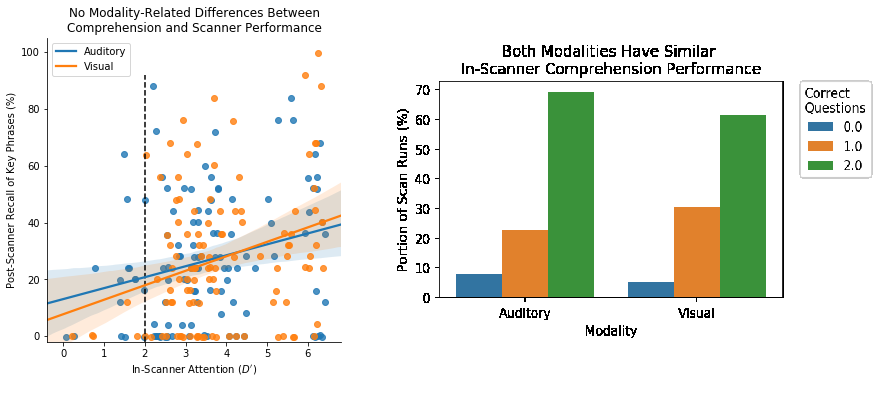
\includegraphics[height=3in]{ch3-task-performance}
    \caption[Behavioral metrics of passage performance were unrelated to modality.]{Both the in-scanner comprehension question and out-of-scanner recall questionnaire were unrelated to the modality of presentation.}
	\label{fig:ch3-task-performance}
\end{figure}

\subsection{Activation results}

A range of language-related areas were activated during reading comprehension (Fig. \ref{fig:ch3-passages-activation-attn}). Compared to the corresponding sensory baselines, activation spanned the inferior frontal gyrus, angular gyrus, premotor cortex, middle temporal gyrus and the superior frontal gyrus. Activation patterns were robustly present on both hemispheres, but had greater intensity and extent on the left hemisphere. 

\begin{figure}[t]
	\centering
	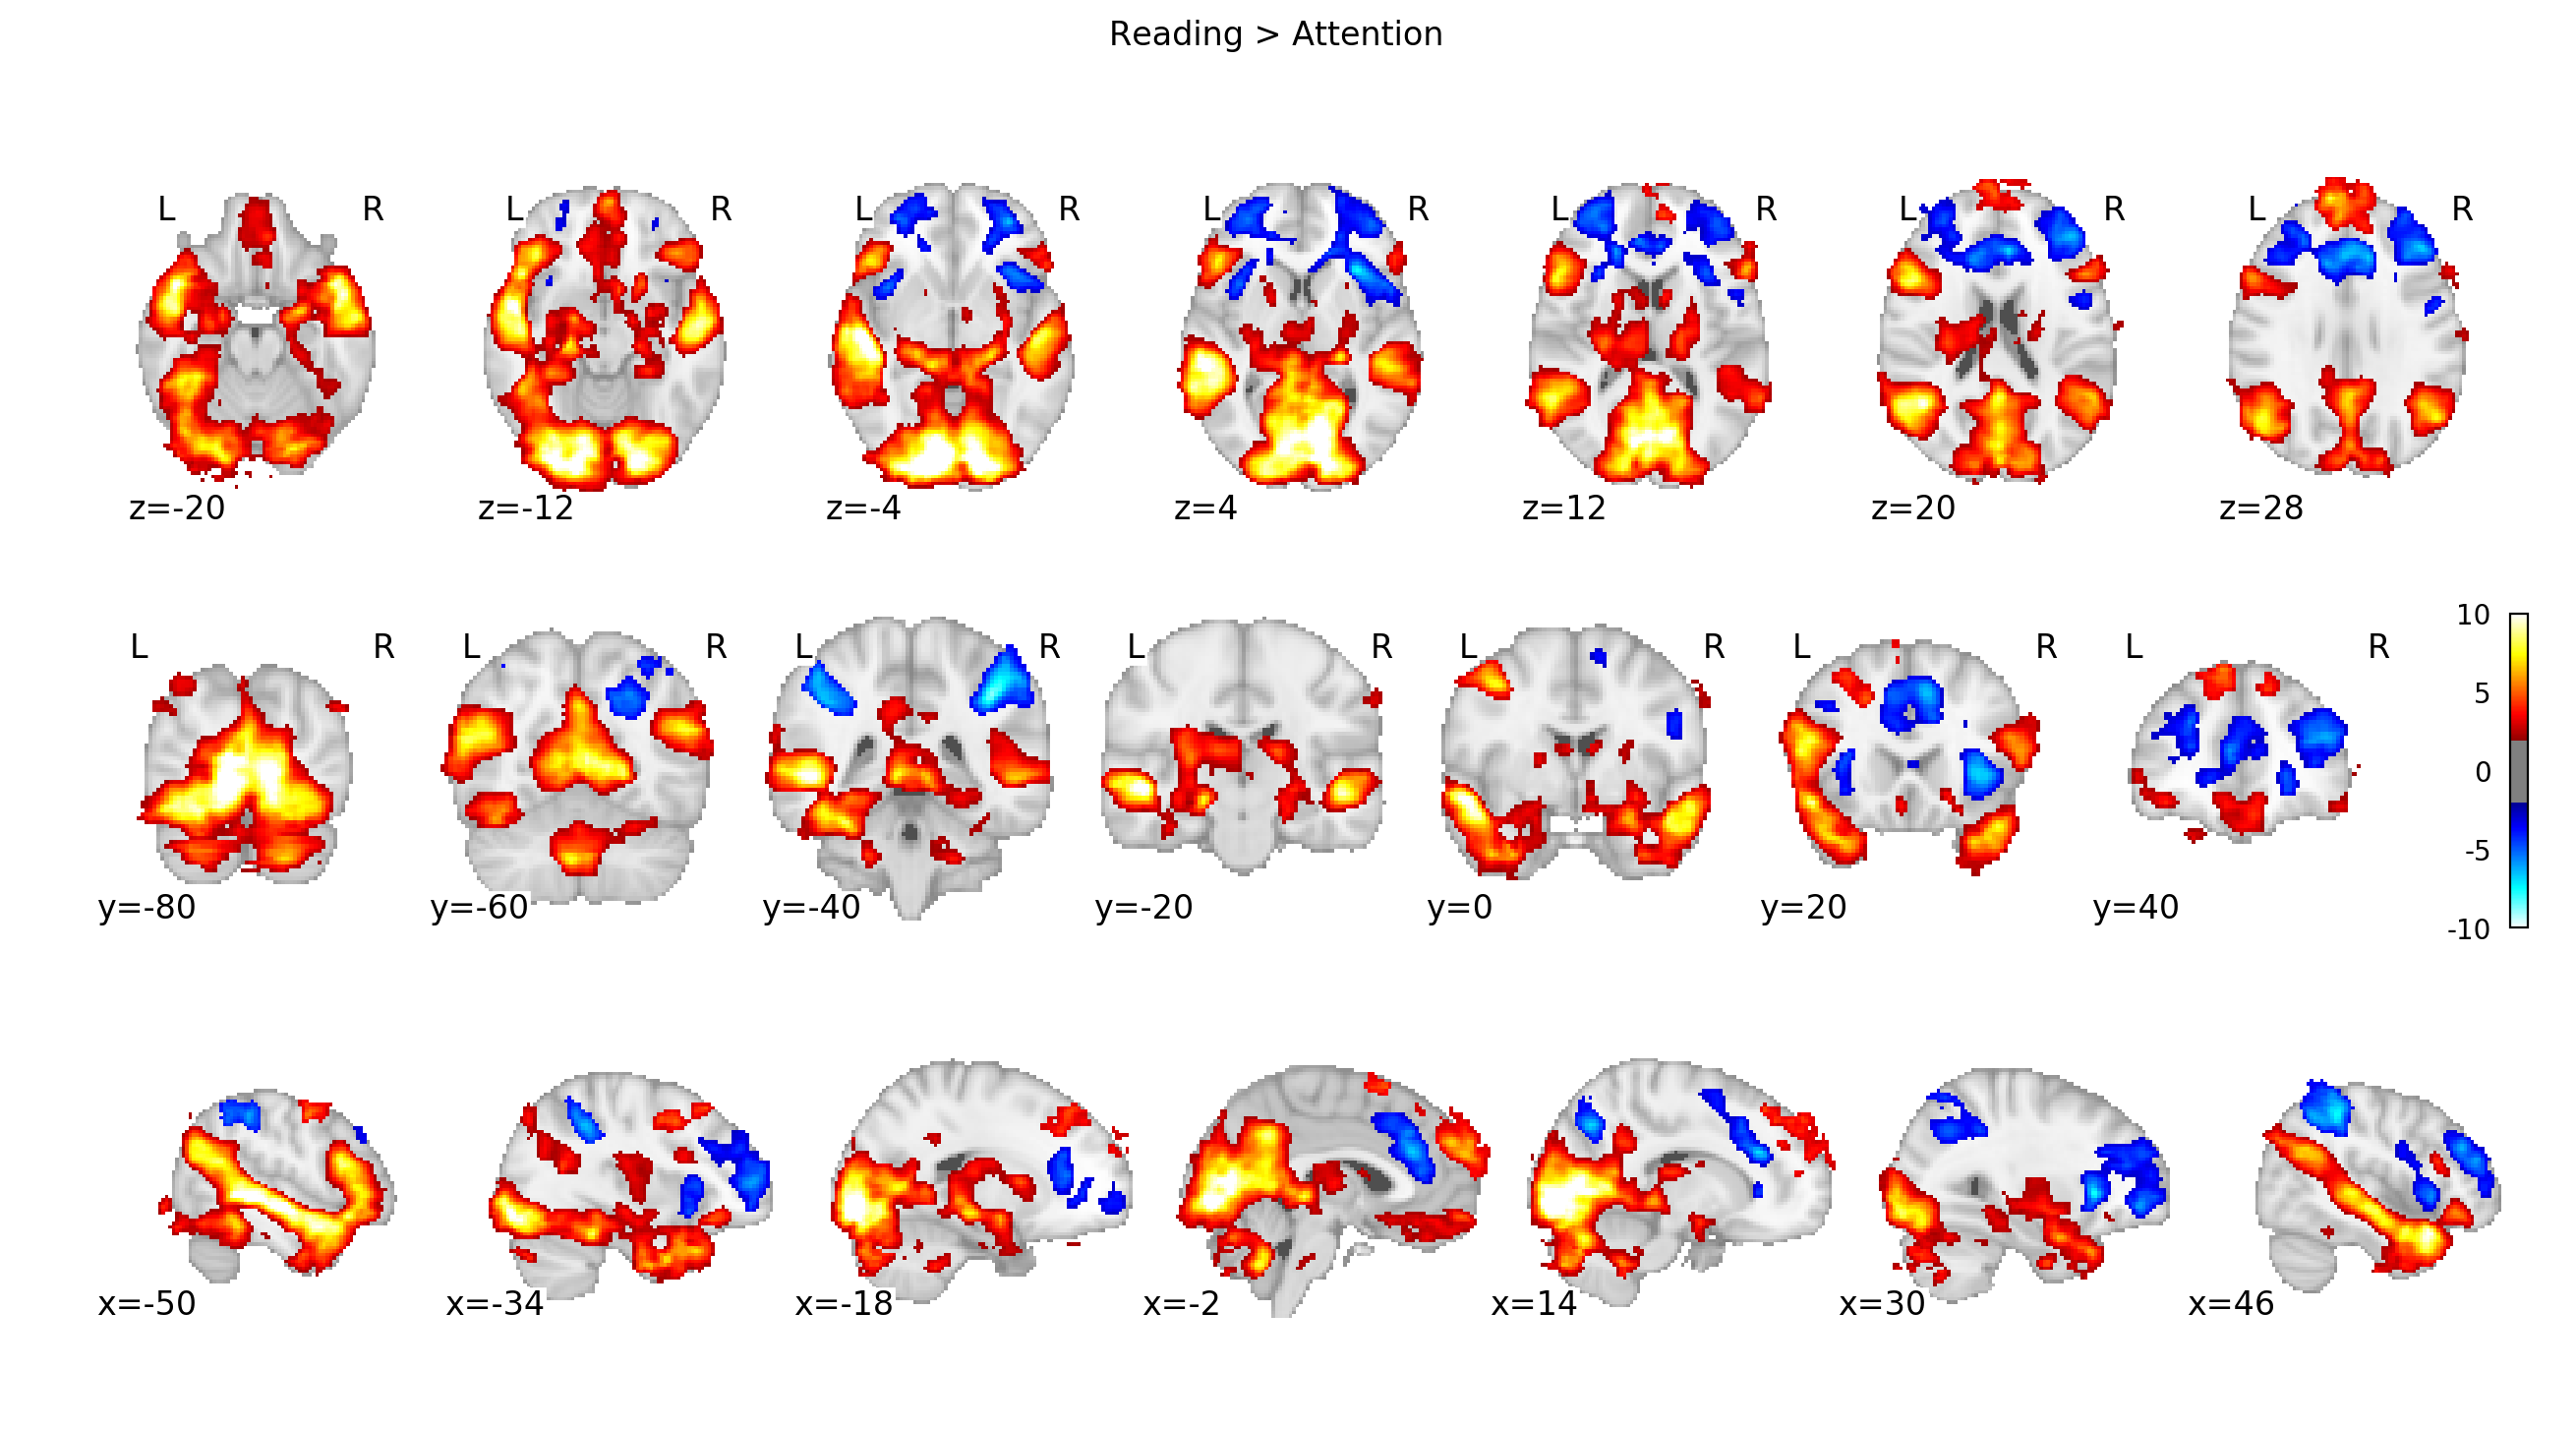
\includegraphics[width=6in]{ch3-reading-brain-activations}
    \caption[A range of language-related areas were activated during reading comprehension.]{A range of language-related areas were activated during reading comprehension. A widespread set of brain areas are utilized during listening and reading, including auditory, default mode and attention areas.}
	\label{fig:ch3-reading-brain-activations}
\end{figure}

We also examined these contrast results when projected onto the 264 nodes in the connectome parcellation. Copmared to the resting baseline, the ventral attention, visual and default mode networks had the greatest number of ``activated'' nodes. It is also notable that the ``uncertain'' nodes were highly engaged, possibly reflecting the important role of functionally diverse regions in the execution of reading comprehension. On the other end, the memory retrieval, salience and cingulo-opercular networks exhibited decreased activity compared to rest. See Fig. \ref{ch3-reading-connectome-activations} for a diagram of these activations by RSN. 

\begin{figure}[t]
	\centering
	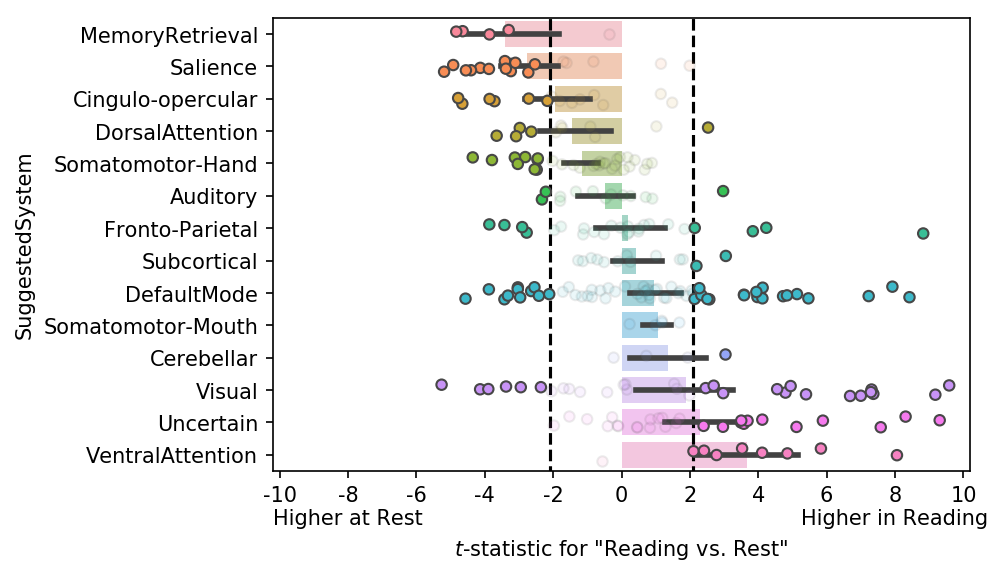
\includegraphics[height=3in]{ch3-reading-connectome-activations}
    \caption[Distribution of reading-related activity among RSN nodes.]{A widespread set of brain areas are utilized during listening and reading, including auditory, default mode and attention areas. Dashed lines represent an uncorrected $p$-value \textless 0.05.}
	\label{fig:ch3-reading-connectome-activations}
\end{figure}


\subsection{Network results}

Next, we examined changes to the global graph theory measures. Figure \ref{fig:ch3-comprehension-graph-theory-all} summarizes the subject-level changes in modularity, participation coefficient, and path length. Overall, the effect was one of increased integration across RSNs during reading comprehension. Relative to rest, both reading comprehension and the sensory baseline reduced the global modularity and increased the participation coefficient, and the magnitude of the effect in reading comprehension was also greater than that of the sensory condition. The path length within each RSN did not significantly change across condition, suggesting that the modular organization of the brain was not disrupted; the RSN parcellation used was still a good fit. However, there were significant increases in the between-RSN path length corresponding to greater efficiency of transferring information between these disparate systems.

\begin{figure}[t]
	\centering
	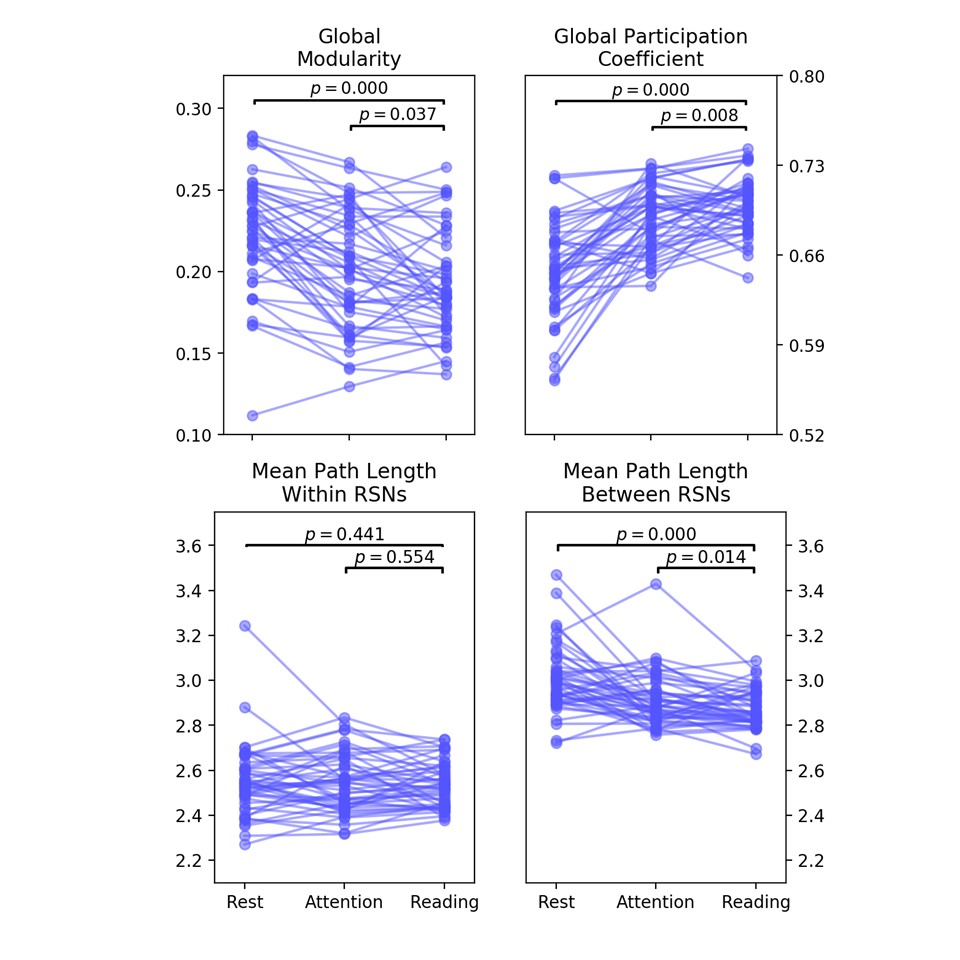
\includegraphics[width=4in]{ch3-comprehension-graph-theory-all}
    \caption[Reading induces more integrated global network architecture.]{Compared to rest and baseline attention tasks, reading comprehension increased measures related to RSN integration.}
	\label{fig:ch3-comprehension-graph-theory-all}
\end{figure}

In general, there was a correlation between greater activity and a greater diversity of connections

% Table summarzing mean activation + GT by RSN ?... 

To investigate interactions between networks, rather than simply general behavior of the networks, we summarized the average shortest path length between each network. This provides a gross measure of how close any two networks are. A node-level diagram of these changes between rest and comprehension is presented in Figure \ref{ch3-modality-node-distance}. 

\begin{figure}[t]
	\centering
	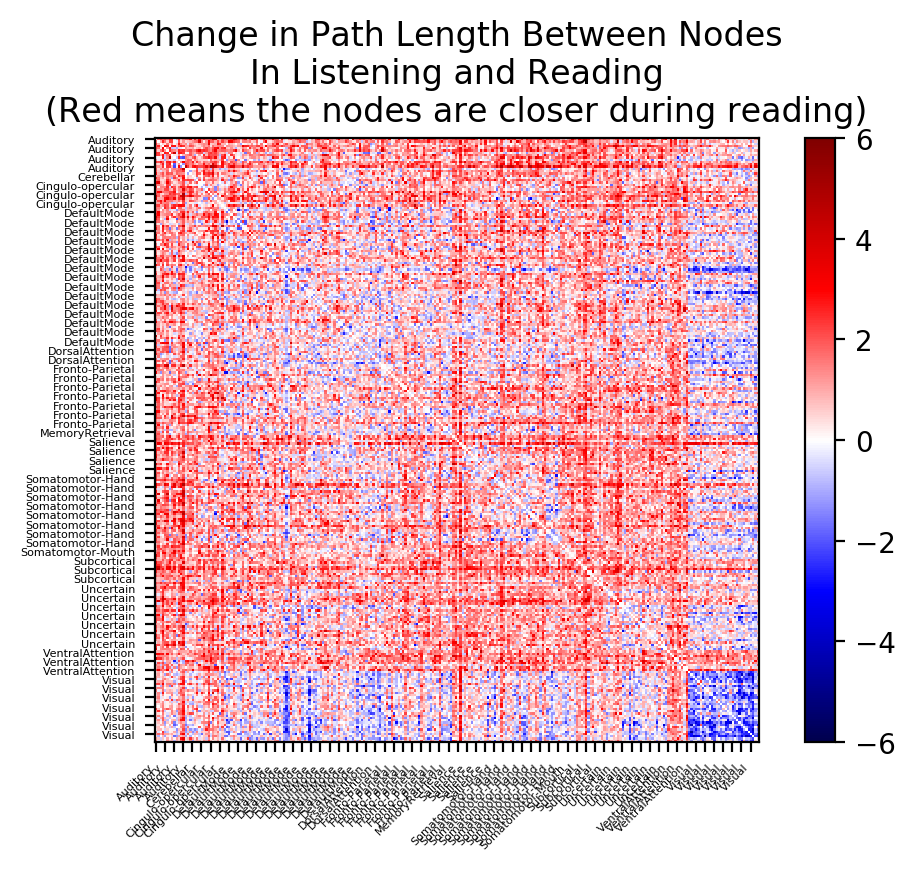
\includegraphics[height=3in]{ch3-modality-node-distance}
    \caption[Language induces more integrated global network architecture.]{Compared to rest and baseline attention tasks, reading and listening increase measures related to global RSN integration.}
	\label{fig:ch3-modality-node-distance}
\end{figure}

Investigating these graph theory measures at the level of RSN provides  insight as to which networks are driving the changes in integration. When comparing comprehension differences to rest, for example, we can see that globally connectivity increases (Fig. \ref{fig:ch3-comprehension-reorganization}. During rest, however, there is increased connectivity within default mode network and visual networks. As would be expected, the visual network undergoes large changes in reading: specifically, there is a large decrease in visual-visual connectivity. 

\begin{figure}[t]
	\centering
	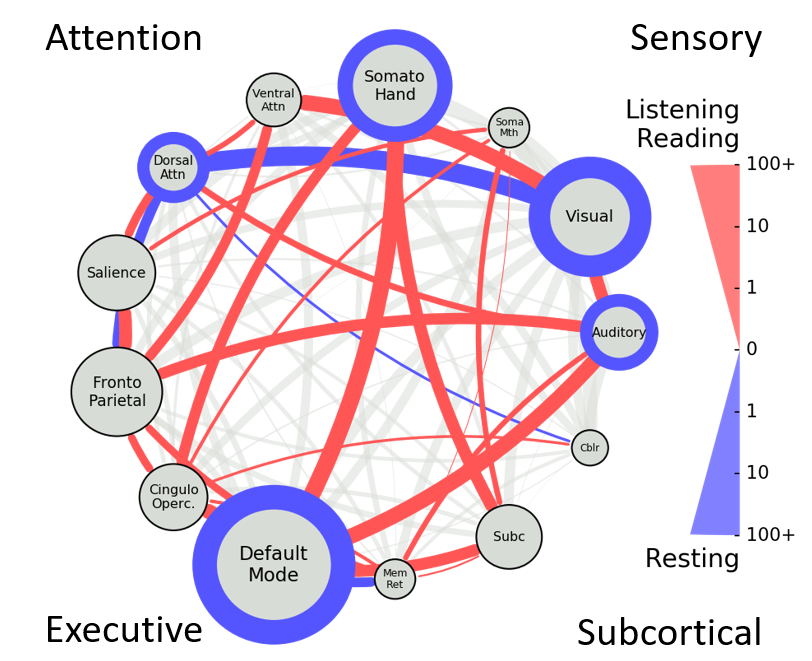
\includegraphics[height=4.5in]{ch3-comprehension-reorganization}
    \caption[Changes in number of connections within and between networks.]{Changes in number of connections within and between networks.}
	\label{fig:ch3-comprehension-reorganization}
\end{figure}

Finally, we sought to address the question of whether better readers more likely to have decreased modularity during reading. As before 

\begin{figure}[t]
	\centering
	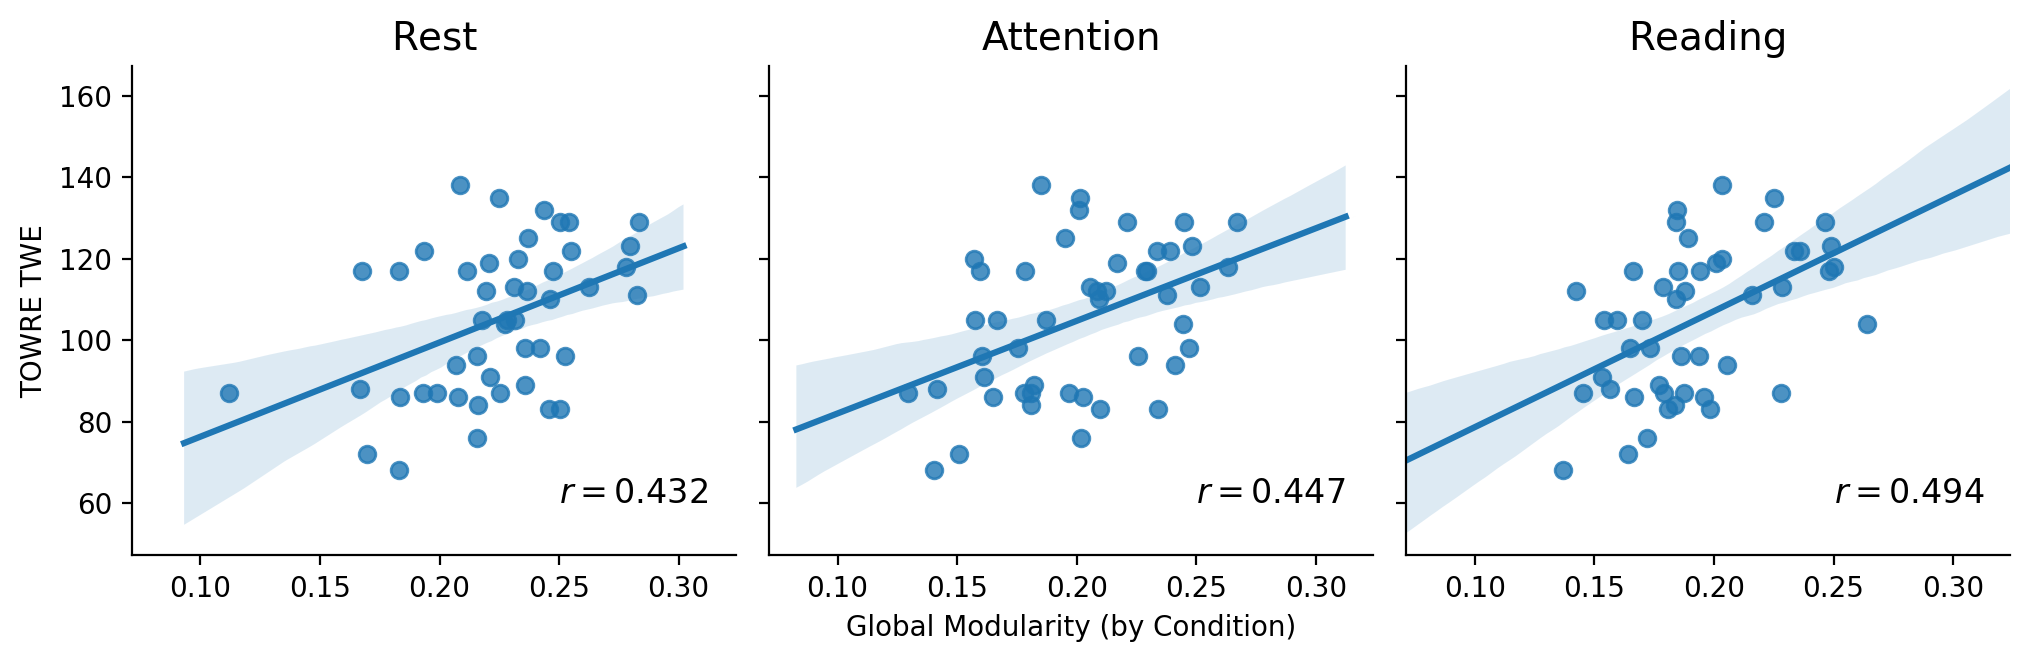
\includegraphics[width=6in]{ch3-modularity-reading-by-condition}
    \caption[Higher modularity in any condition is related to reading skill.]{Higher modularity in any condition is related to reading skill. Greater integration between}
	\label{fig:ch3-modularity-reading-by-condition}
\end{figure}


\section{Discussion}

This study investigates the differences between reading and listening in terms of their activation of individual areas or the distribution of activity across the brain. We employ closely matched texts, large sample size, longitudinal sampling, and behavioral covariates. Comprehending extended text requires more than just sensory and linguistic processes. It also requires executive processes such as attention, working memory and inference. Since comprehension is a "whole-brain" activity, we here look at the reorganization of resting-state networks - to see how attention, executive and sensory systems are interacting during reading.

The results make clear that differences in reading are not isolated solely to sensory systems, although the visual system is the major driver. We tested three hypotheses related to global reorganization, sensory system changes, and interactions between executive and attention systems and sensory systems.

These modality-specific influences on behavior and brain activity may arise from a few different sources: subject, linguistic and innate differences. For example, there are also differences in what is encoded in speech and text. The reading sciences pioneer Alvin Liberman noted that "speech is a complex code, while reading is a simple cipher" \cite{Mattingly1971}. Speech contains overt clues about the speaker, such as tone and prosody, and these can convey additional non-linguistic meaning for the listener. Reading, on the other hand, might be considered a more purely linguistic act, especially with computer-printed text. Reading may thus allow more room for self-generated situation models and more independent direction of thought. Furthermore, modality-specific aspects of the stimulus may influence the overall comprehension process; reading requires a level of spatial awareness -where one is at on a page, what happened in preceding paragraphs – and allows for the re-treading of information. Listening, meanwhile, requires the extraction of input from competing noises and sometimes the tracking of changing volume. 

People speak differently than they write. Reading often relies on more complicated syntax, and even for skilled readers, longer words and sentences can strain executive systems more than they might if being spoken to. Although these properties are often controlled for in scientific studies, they represent a major difference between “natural” reading and listening. Because of these differences, reading may place a greater load on executive function skills. Executive functions such as working memory and planning and organizing may be particularly important for reading \citep{Cain2006}.  

The last set of differences is particularly interesting because knowing how the differences in reading interact with these modality differences. Reading is a learned skill with may component processes. It requires thousands of hours of experience to master and entails a reorganization of cortical resources. Environmental and biological factors thus exert a greater influence on an individual’s reading proficiency than they might on more intrinsic processes such as speech comprehension. This is particularly dramatic in individuals with dyslexia, who have persistent difficulty with reading. Children with dyslexia exhibit less activation in reading-related areas compared to typically developing children \citep{Pugh2000}, but greater activation in right hemisphere homologues, suggesting that lateralization and activation of the reading circuit are associated with better reading. Development period also has an effect, with children exhibiting less activation in frontal areas but more in posterior areas, possibly reflecting a shift in “resource load” from uni-modal to supramodal areas \citep{Berl2011}. This shift may not be necessary in listening, or occur much earlier. Thus, with increasing expertise and development, there may be a “shift” from relying on fusiform processing areas. towards using multi-modal areas more like speech \citep{Monzalvo2013}. 

This interaction between reading activation and individual differences in maturity and reading skill will be the subject of the next chapter.